\section{Backend Projekt-Überblick}
\setauthor{Sebastian Egger}

Das Backend setzt sich aus 9 Projekten zusammen, welche in C\# .Net 5 entwickelt wurden.


\begin{figure}[H]
    \centering
    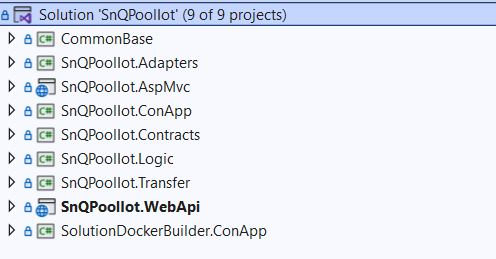
\includegraphics[width=0.7\textwidth]{pics/Projektmappe.JPG}
    \caption{Projektmappe}
\end{figure}


\begin{itemize}
    \item CommonBase
    \\
    In CommonBase befinden sich Klassen und Methoden, die wiederverwendbar sind, um Codeverdoppelung zu vermeiden.
\end{itemize}


\begin{itemize}
    \item SnQPoolIot.Adapters
    \\
    SnQPoolIot.Adapters bietet einen direkten Zugriff auf die Logic.
Der Zugriff auf die Logic kann dadurch entweder direkt erfolgen oder per Rest über die WebApi.
\end{itemize}

\begin{itemize}
    \item SnQPoolIot.WebApi
    \\
    Der Zugriff auf die Messwerte wird durch Rest-Zugriffe in SnQPoolIot.WebApi provided.
    Auf die Daten kann aber nur per Login mit einem gültigen Account zugegriffen werden.
    Genaueres zu den einzelnen HTTP-Requests ist im Kapitel HTTP und Verwendung in unserem Backend zu finden.
\end{itemize}

\begin{itemize}
    \item SnQPoolIot.Contracts
    \\
    SnQPoolIot.Contracts beinhaltet alle notwendigen Schnittstellen und Enumerationen des Projektes.
    Hier werden die Entitäten als Interfaces angelegt.
\end{itemize}


\begin{itemize}
    \item SnQPoolIot.Logic
    \\
    SnQPoolIot.Logic ist das Kernstück des Projektes. 
    Durch die Logic können alle Daten aus der Datenbank verwendet werden. 
    Die Logik verbindet sich mit einer Sqlite Datenbank. Der Zugriff und das Erzeugen der Datenbank wird mittels Entityframework.Sqlite durchgeführt.
\end{itemize}

\begin{itemize}
    \item SnQPoolIot.Transfer
    SnQPoolIot.Transfer verwaltet die Transferobjekte für den Datenaustausch zwischen den Layern.
\end{itemize}


\begin{itemize}
    \item SnQPoolIot.AspMvc
    SnQPoolIot.AspMvc ist ein Ersatz für das Frontend.
    Hier werden die Funktionen z.B.: das Einloggen eines Users oder Anzeigen von Messwerten dargestellt.
\end{itemize}

\begin{itemize}
    \item SnQPoolIot.ConApp
    In SnQPoolIot.ConApp werden User mit verschiedenen Rechten angelegt, die für die Authentifizierung benötigt werden.
\end{itemize}




\subsection{SnQPoolIot.WebApi}

\subsubsection*{HTTP und Verwendung im Backend}

HTTP ausgeschrieben Hypertext Transfer Protocoll wird zum Laden von Webseiten im Projekt verwendet.
Die verwendeten HTTP-Requests und das dazugehörige Routing ist im Projekt SnQPoolIot.WebApi implementiert.

Hier ein Ausschnitt von dem Aufbau der WebApi:

\begin{figure}[H]
    \centering
    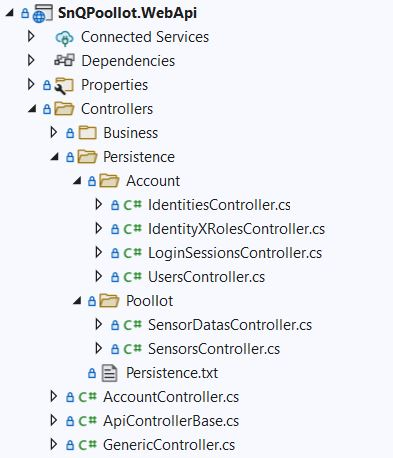
\includegraphics[width=1\textwidth]{pics/HTTPRequestsWebApi.JPG}
    \caption{Aufbau der WebApi}
\end{figure}


Das Routing der Websiten wird über die Controller gemanaged. 
Der meist genützte Controller in diesem Projekt ist der GenericController, denn er bietet allen abgeleiteten Controllern seine bereitgestellten Funktionen zur Verwendung an.

\begin{figure}[H]
    \centering
    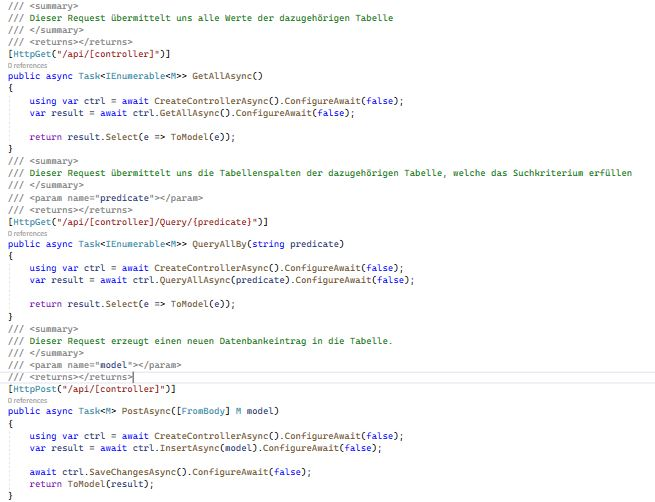
\includegraphics[width=1\textwidth]{pics/GenericControllerWebApi.JPG}
    \caption{Auszug GenericController der WebApi}
\end{figure}

Wie am Beispiel des Codeauszuges zu sehen, beinhaltet der Generic Controller einige Methoden.
Für die Ermittlung der Daten wird zum Beispiel eine Get-Methode "GetAllAsync" eingesetzt.
Die Codezeile [HttpGet("/api/[controller]")] drückt aus, dass es sich bei dieser Methode um eine Get-Methode handelt und veranschaulicht auch das Routing der WebApi.
All jene Methoden, die im GenericController definiert sind stehen demnach allen von ihm abgeleiteten Controllern zur Verfügung und können direkt verwendet werden.

Im nachstehenden Beispiel wird eine Ableitung vom GenericController dargestellt.

\begin{figure}[H]
    \centering
    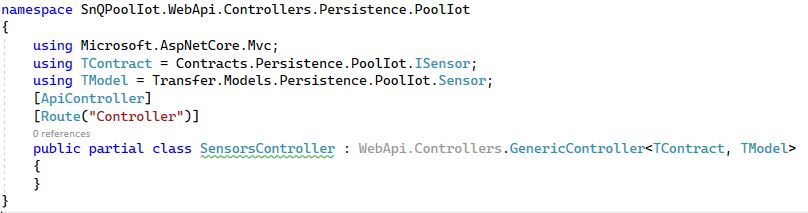
\includegraphics[width=0.7\textwidth]{pics/VerwendungGenereicController.JPG}
    \caption{Anwendung des GenericControllers der WebApi}
\end{figure}


\subsubsection*{Verwendung von Swagger im Projekt}
Zum Allgemeinen Überblick aller HTTP-Requests wird Swagger verwendet.

\begin{figure}[H]
    \centering
    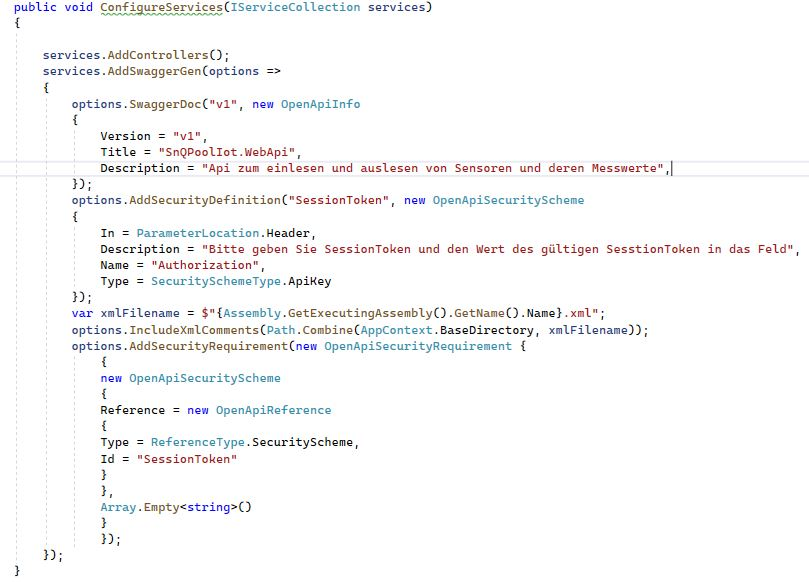
\includegraphics[width=0.8\textwidth]{pics/SwaggerImplementation.JPG}
    \caption{Implementierung von Swagger in der WebApi}
\end{figure}

In den nachstehenden Zeilen findet sich eine kurze Ablaufbeschreibung des Codes:
Sobald die Methode ConfigureServices aufgerufen wird, wird dem service ein neuer Controller angelegt und die benötigte Konfiguration des Swaggers mit übergeben. 

Das options.SwaggerDoc gibt eine kurze Beschreibung über die WebApi an.
Im darauf folgenden Schritt wird die Authentifizierung im Projekt mittels Swagger durchgeführt. Dadurch wird gewährleistet, dass nur eingeloggte Benutzer die Möglichkeit haben Zugriffe auf HTTP-Requests durchzuführen.
Sobald die Methode fertig ausgeführt wurde startet im Browser eine Website mit allen HTTP-Requests die im Projekt implementiert sind.

\subsubsection*{Unterstützte HTTP-Requests des Projektes}
Mit Hilfe von Swagger wurden die in den nachstehenden Grafiken ersichtlichen HTTP-Requests des Backends dokumentiert:

\begin{figure}[H]
    \flushleft
    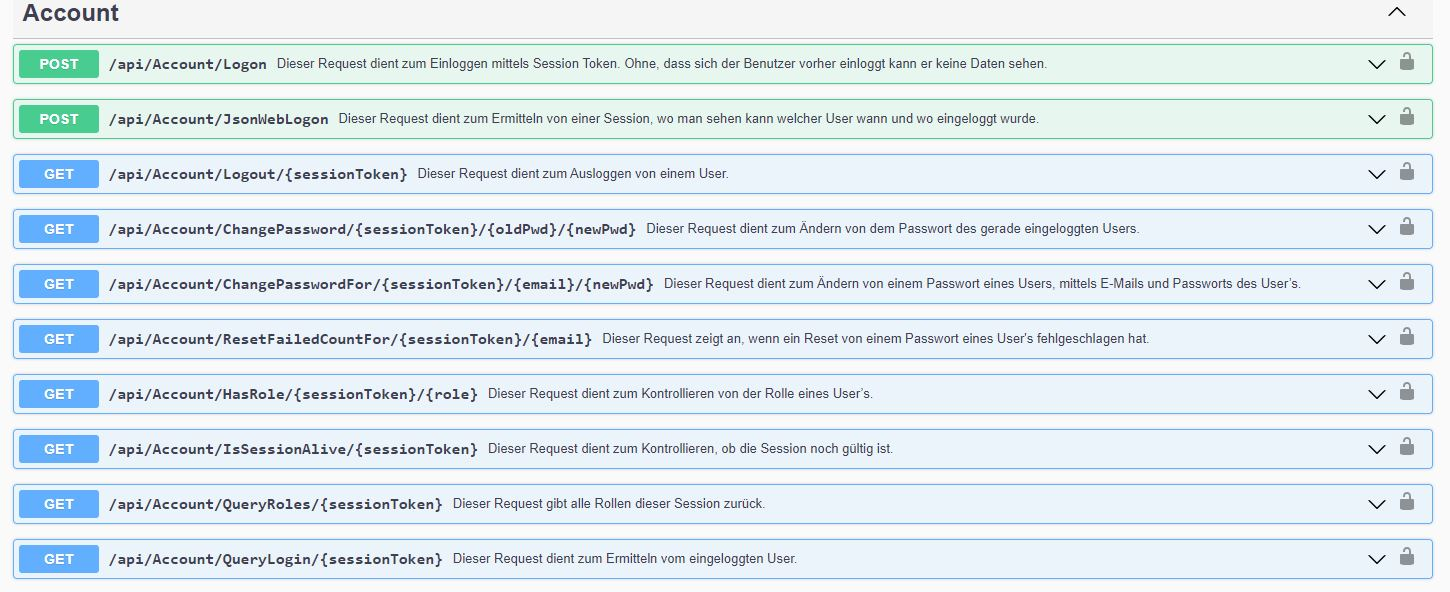
\includegraphics[width=1.6\textwidth]{pics/WebApiRequests1.JPG}
    \caption{HTTP-Requests des Projektes}
\end{figure}

\begin{figure}[H]
    \centering
    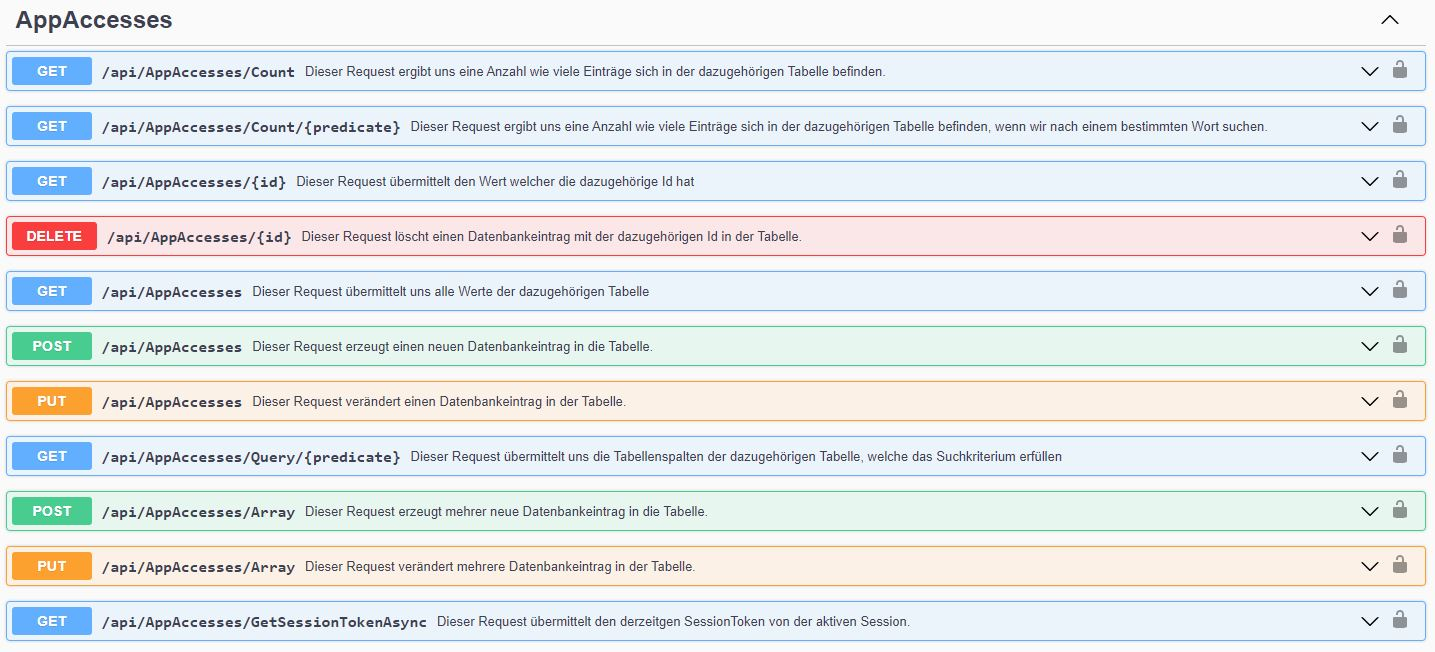
\includegraphics[width=1.6\textwidth]{pics/WebApiRequests2.JPG}
    \caption{HTTP-Requests des Projektes}
\end{figure}

\begin{figure}[H]
    \centering
    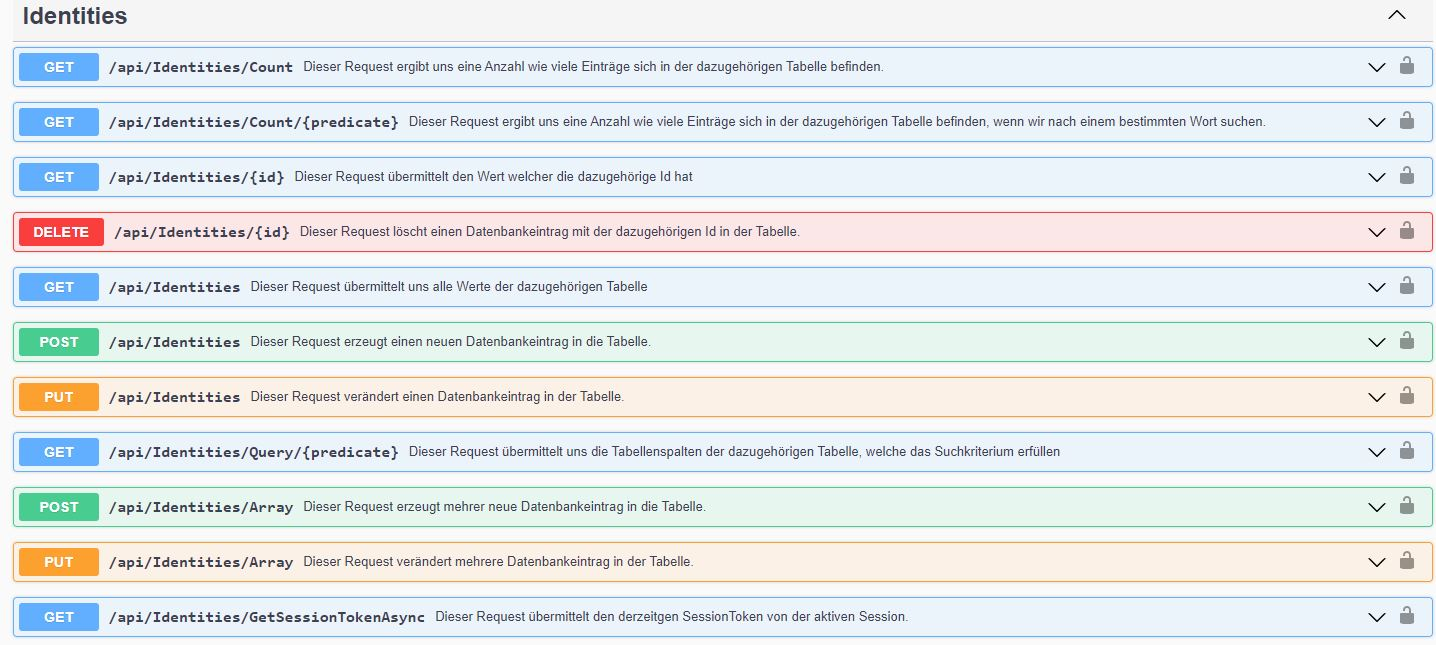
\includegraphics[width=1.6\textwidth]{pics/WebApiRequests3.JPG}
    \caption{HTTP-Requests des Projektes}
\end{figure}

\begin{figure}[H]
    \centering
    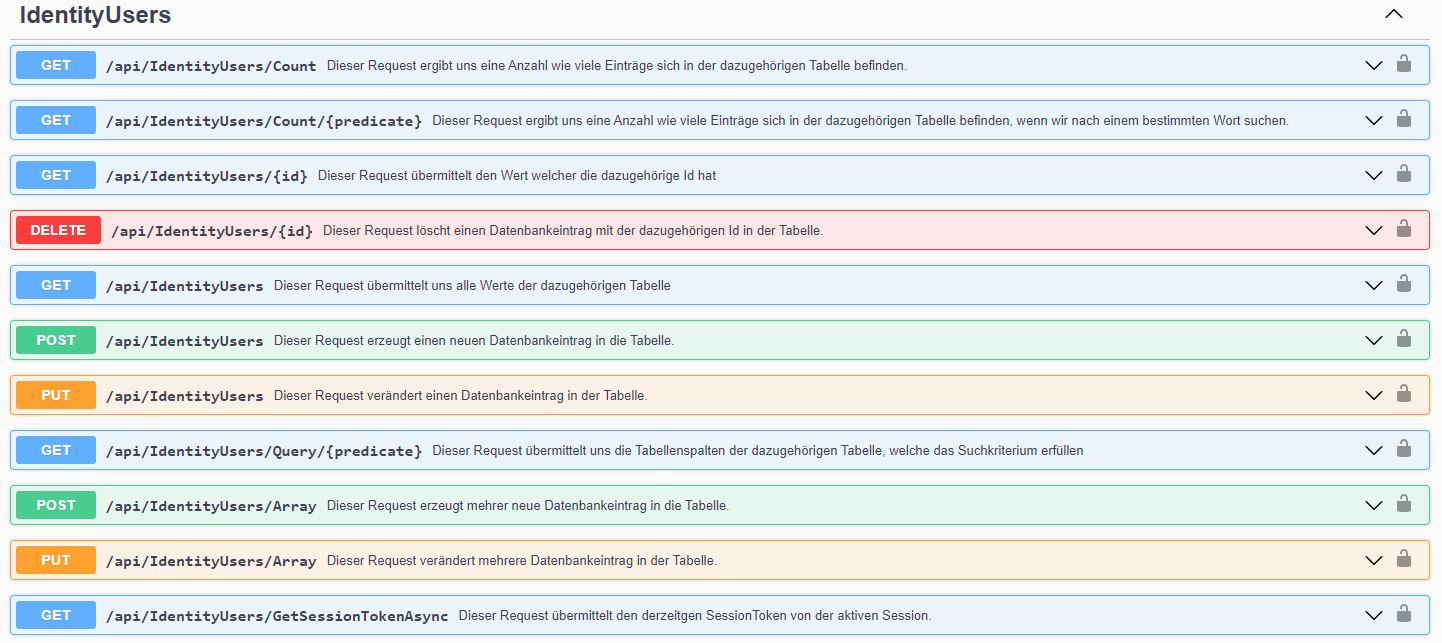
\includegraphics[width=1.6\textwidth]{pics/WebApiRequests4.JPG}
    \caption{HTTP-Requests des Projektes}
\end{figure}

\begin{figure}[H]
    \centering
    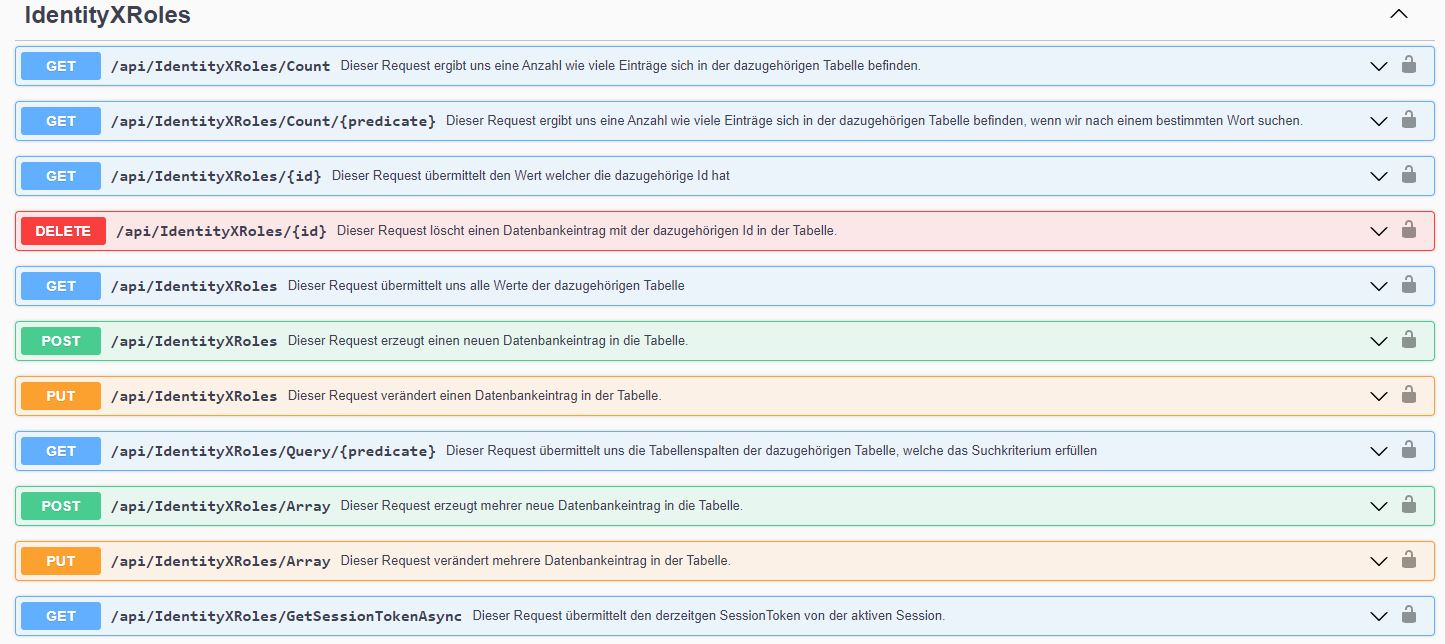
\includegraphics[width=1.6\textwidth]{pics/WebApiRequests5.JPG}
    \caption{HTTP-Requests des Projektes}
\end{figure}

\begin{figure}[H]
    \centering
    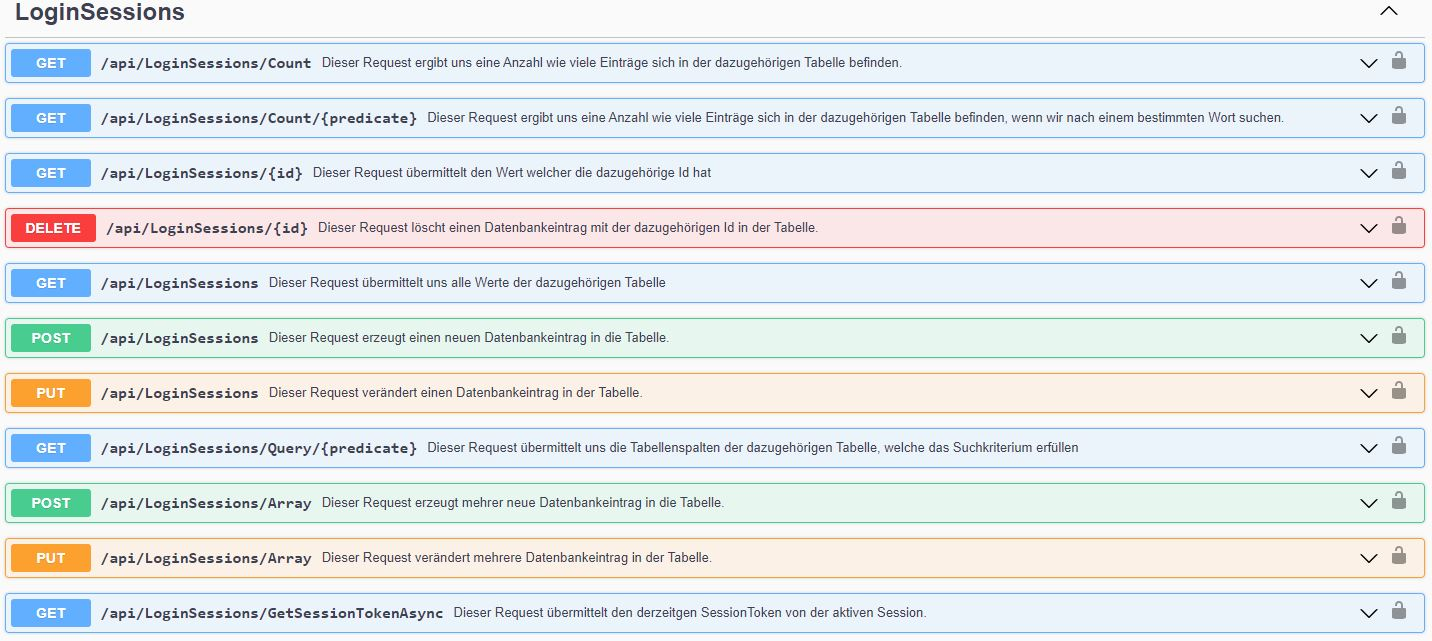
\includegraphics[width=1.6\textwidth]{pics/WebApiRequests6.JPG}
    \caption{HTTP-Requests des Projektes}
\end{figure}

\begin{figure}[H]
    \centering
    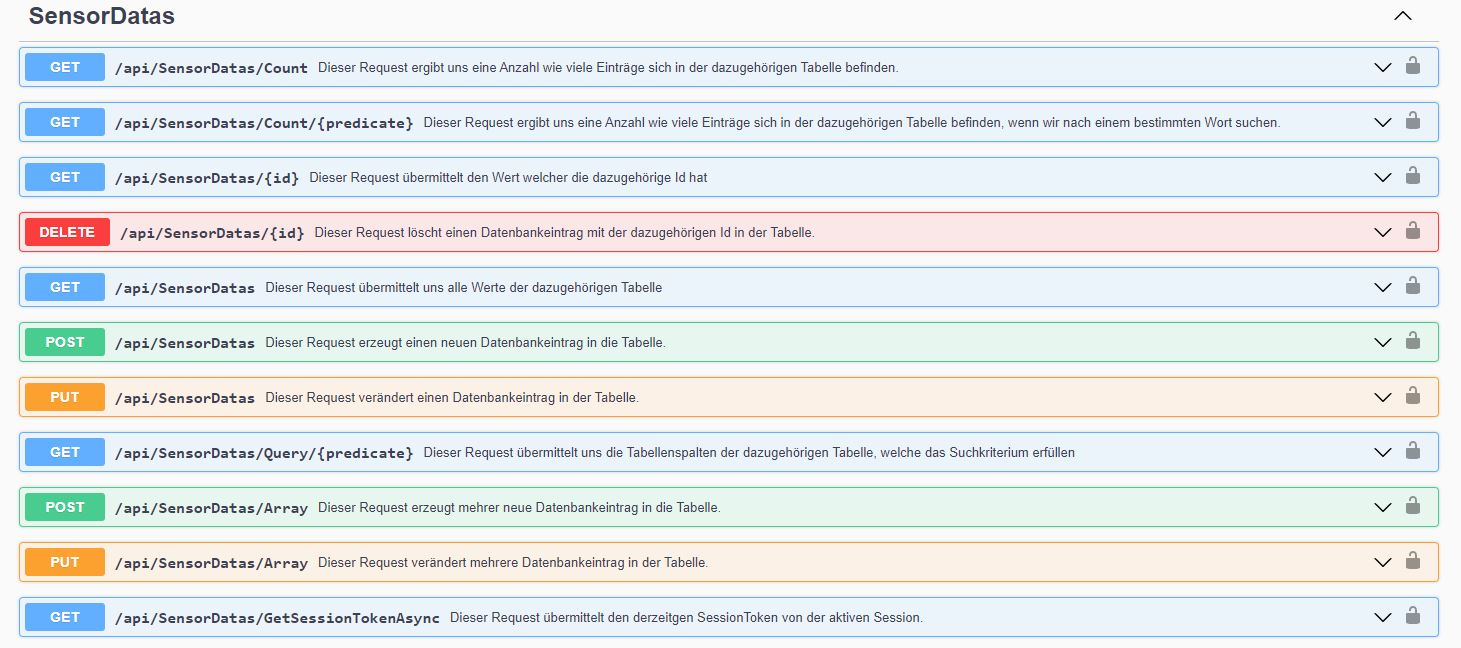
\includegraphics[width=1.6\textwidth]{pics/WebApiRequests7.JPG}
    \caption{HTTP-Requests des Projektes}
\end{figure}

\begin{figure}[H]
    \centering
    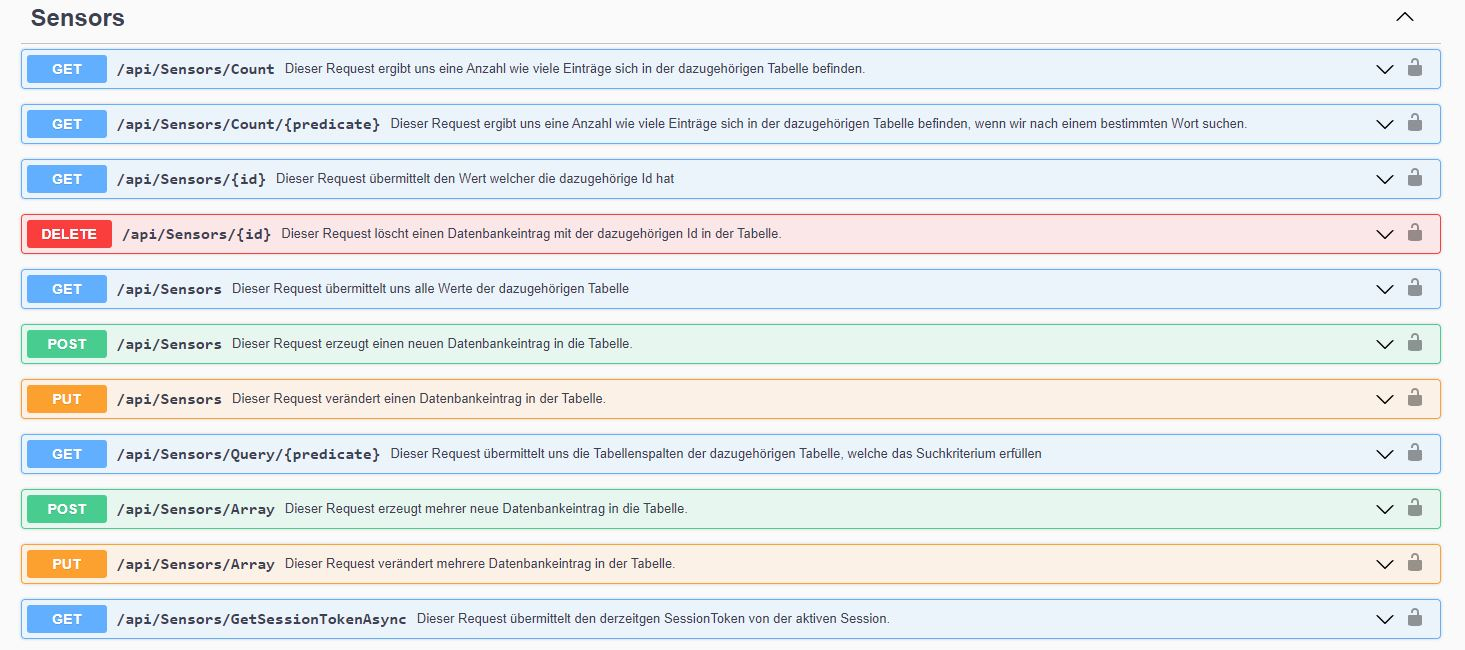
\includegraphics[width=1.6\textwidth]{pics/WebApiRequests8.JPG}
    \caption{HTTP-Requests des Projektes}
\end{figure}

\begin{figure}[H]
    \centering
    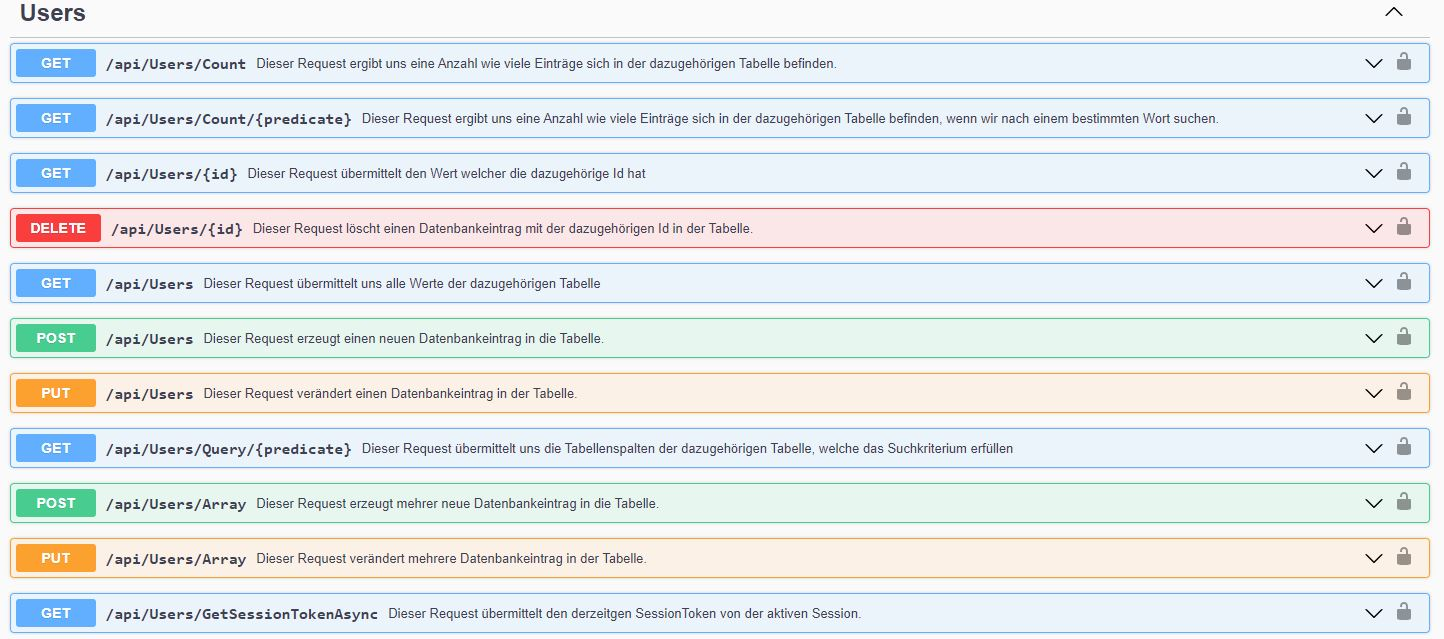
\includegraphics[width=1.6\textwidth]{pics/WebApiRequests9.JPG}
    \caption{HTTP-Requests des Projektes}
\end{figure}


\subsection{SnQPoolIot.Logic}
Wie  bereits im Backend Projekt-Überblick beschrieben, befindet sich in SnQPoolIot.Logic die Datenbank mit den Zugriffen.
Die Datenbank wird mithilfe des NuggetPackage Microsoft.Entityframework.Sqlite, den Befehlen:
dotnet ef migrations add InitDb und dotnet ef database update, welche in der Developer-PowerShell 
im Visual Studio ausgeführt werden müssen um Migrations zu erzugen und um die Datenbank mit den erzeugten Migrations upzudaten, 
und einem DBContext, welcher die Configuration der Datenbank mit sich bringt, automatisch erstellt. 

\begin{figure}[H]
    \centering
    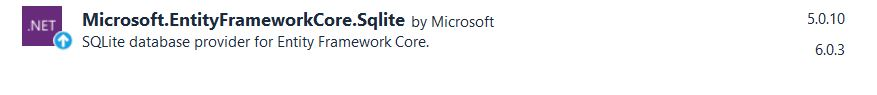
\includegraphics[width=1\textwidth]{pics/EntityFrameworkSqlLiteNuggetPackage.JPG}
    \caption{NuggetPackage für Entityframework mit Sqlite}
\end{figure}


\begin{figure}[H]
    \centering
    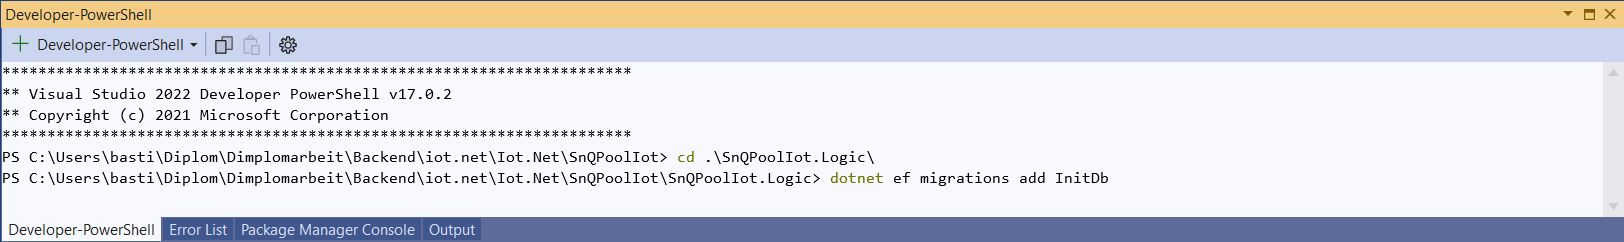
\includegraphics[width=1\textwidth]{pics/DeveloperPowerShellMigration.JPG}
    \caption{Befehl zum Erzeugen von Migationen}
\end{figure}

\begin{figure}[H]
    \centering
    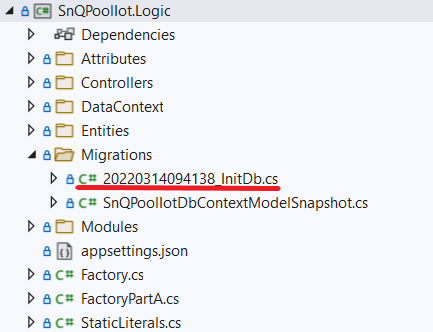
\includegraphics[width=1\textwidth]{pics/MigrationCreated.png}
    \caption{Erzeugte Migrationen in der Logik}
\end{figure}

\begin{figure}[H]
    \centering
    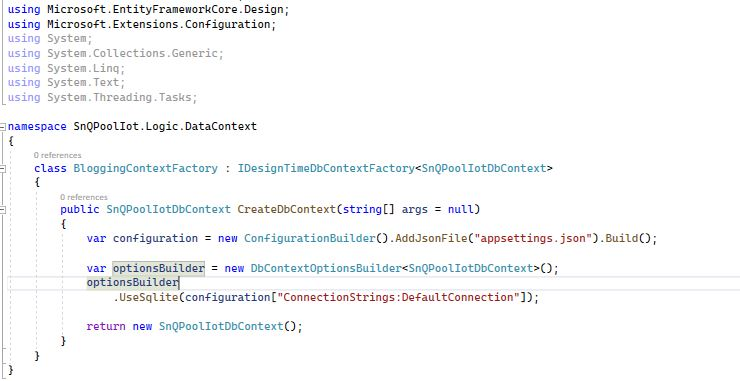
\includegraphics[width=1\textwidth]{pics/DBContext.JPG}
    \caption{DBContext zum Erzeugen einer Datenbank}
\end{figure}

Nun zu den Datenbank Zugriffen. Damit auf die Messwerte zugegriffen werden kann muss sich ein User zuerst authentifizieren.
Damit sich eine User authentifizieren kann benötigt er einen Account mit E-Mail und Passwort, welche in der Datenbank gespeichert sind.
Für die Authentifizierung werden die nachstehenden Tabellen benötigt:

\begin{itemize}
    \item Identity
    In dieser Tabelle befinden sich alle User-Accounts mit E-Mail gehastem Passwort.

    \begin{figure}[H]
        \centering
        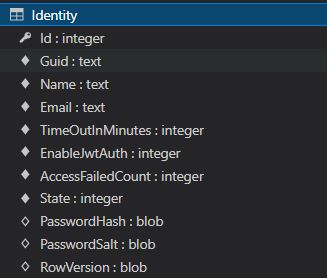
\includegraphics[width=0.7\textwidth]{pics/IdentityTableStructur.JPG}
        \caption{Identity Tabelle mit den dazugehörigen Tabellenspalten}
    \end{figure}

\end{itemize}


\begin{itemize}
    \item Role
    In dieser Tabelle sind alle Rollen die es gibt vorzufinden.

    \begin{figure}[H]
        \centering
        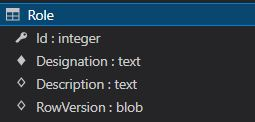
\includegraphics[width=1\textwidth]{pics/RoleTableStructure.JPG}
        \caption{Role Tabelle mit den dazugehörigen Tabellenspalten}
    \end{figure}

\end{itemize}

\begin{itemize}
    \item IdentityXRole
    Diese Tabelle weißt einem Benutzer eine Rolle zu.
    \begin{figure}[H]
        \centering
        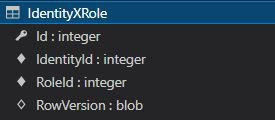
\includegraphics[width=1\textwidth]{pics/IdentityXRoleStructure.JPG}
        \caption{IdentityXRole Tabelle mit den dazugehörigen Tabellenspalten}
    \end{figure}
\end{itemize}


\begin{itemize}
    \item LogginSession
    Diese Tabelle zeigt alle Logins mit dem dazugehörigen User und den SessionToken mit dem sich der User eingeloggt hat an.
    \begin{figure}[H]
        \centering
        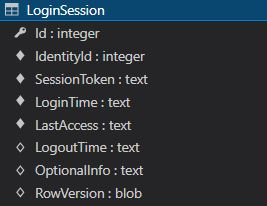
\includegraphics[width=1\textwidth]{pics/LoginSessionStructure.JPG}
        \caption{LogginSession Tabelle mit den dazugehörigen Tabellenspalten}
    \end{figure}
\end{itemize}

Sobald sich ein User authentifitiert hat wurde zugleich eine neue Session erstellt und wenn die Rechte vom
dem authentifizierten User hochgenug sind kann er sich nun die Messwerte ansehen.
Die nachstehenden Tabellen dienen zum Erfassen von den Messwerten:

\begin{itemize}
    \item Sensor
    Diese Tabelle beinhaltet den Namen eines Sensors.
    \begin{figure}[H]
        \centering
        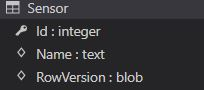
\includegraphics[width=1\textwidth]{pics/SensorTableStructure.JPG}
        \caption{Sensor Tabelle mit den dazugehörigen Tabellenspalten}
    \end{figure}
\end{itemize}

\begin{itemize}
    \item Sensor
    Diese Tabelle beinhaltet die Messwerte aller Sensoren und beinhaltet welcher Messwert zu welchen Sensor gehört.
    \begin{figure}[H]
        \centering
        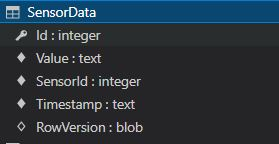
\includegraphics[width=1\textwidth]{pics/SensorDataTableStructure.JPG}
        \caption{SensorData Tabelle mit den dazugehörigen Tabellenspalten}
    \end{figure}
\end{itemize}


\subsubsection*{Logging in unserem Projekt}


\subsection{SnQPoolIot.AspMvc}

